
\chapter{Aufgabe D3}

\section{Simulink-Modell}
Die nachfolgenden Abbildungen zeigen das Simulink-Modell zur Berechnung der Distanzen der einzelnen Räder.\\
Das Modell in \autoref{fig:drivingdistances1} hat die vier Geschwindigkeiten (in km/h) der Räder als Eingänge. Diese werden mit dem \glqq From Workspace"' Block mit ihrer zugehöhrigen Referenzzeit tv in das Model importiert.\\
Danach werden sie in m/s umgerechnet und integriert, um die Strecke zu erhalten. \\
Zur Simulation wird ein FixedStep von 0.01 mit dem ode3-Solver verwendet. Der ode-Solver wurde durch die Simulink \glqq automatic solver selection"' ausgewählt.
\begin{figure}[h!]
	\centering
	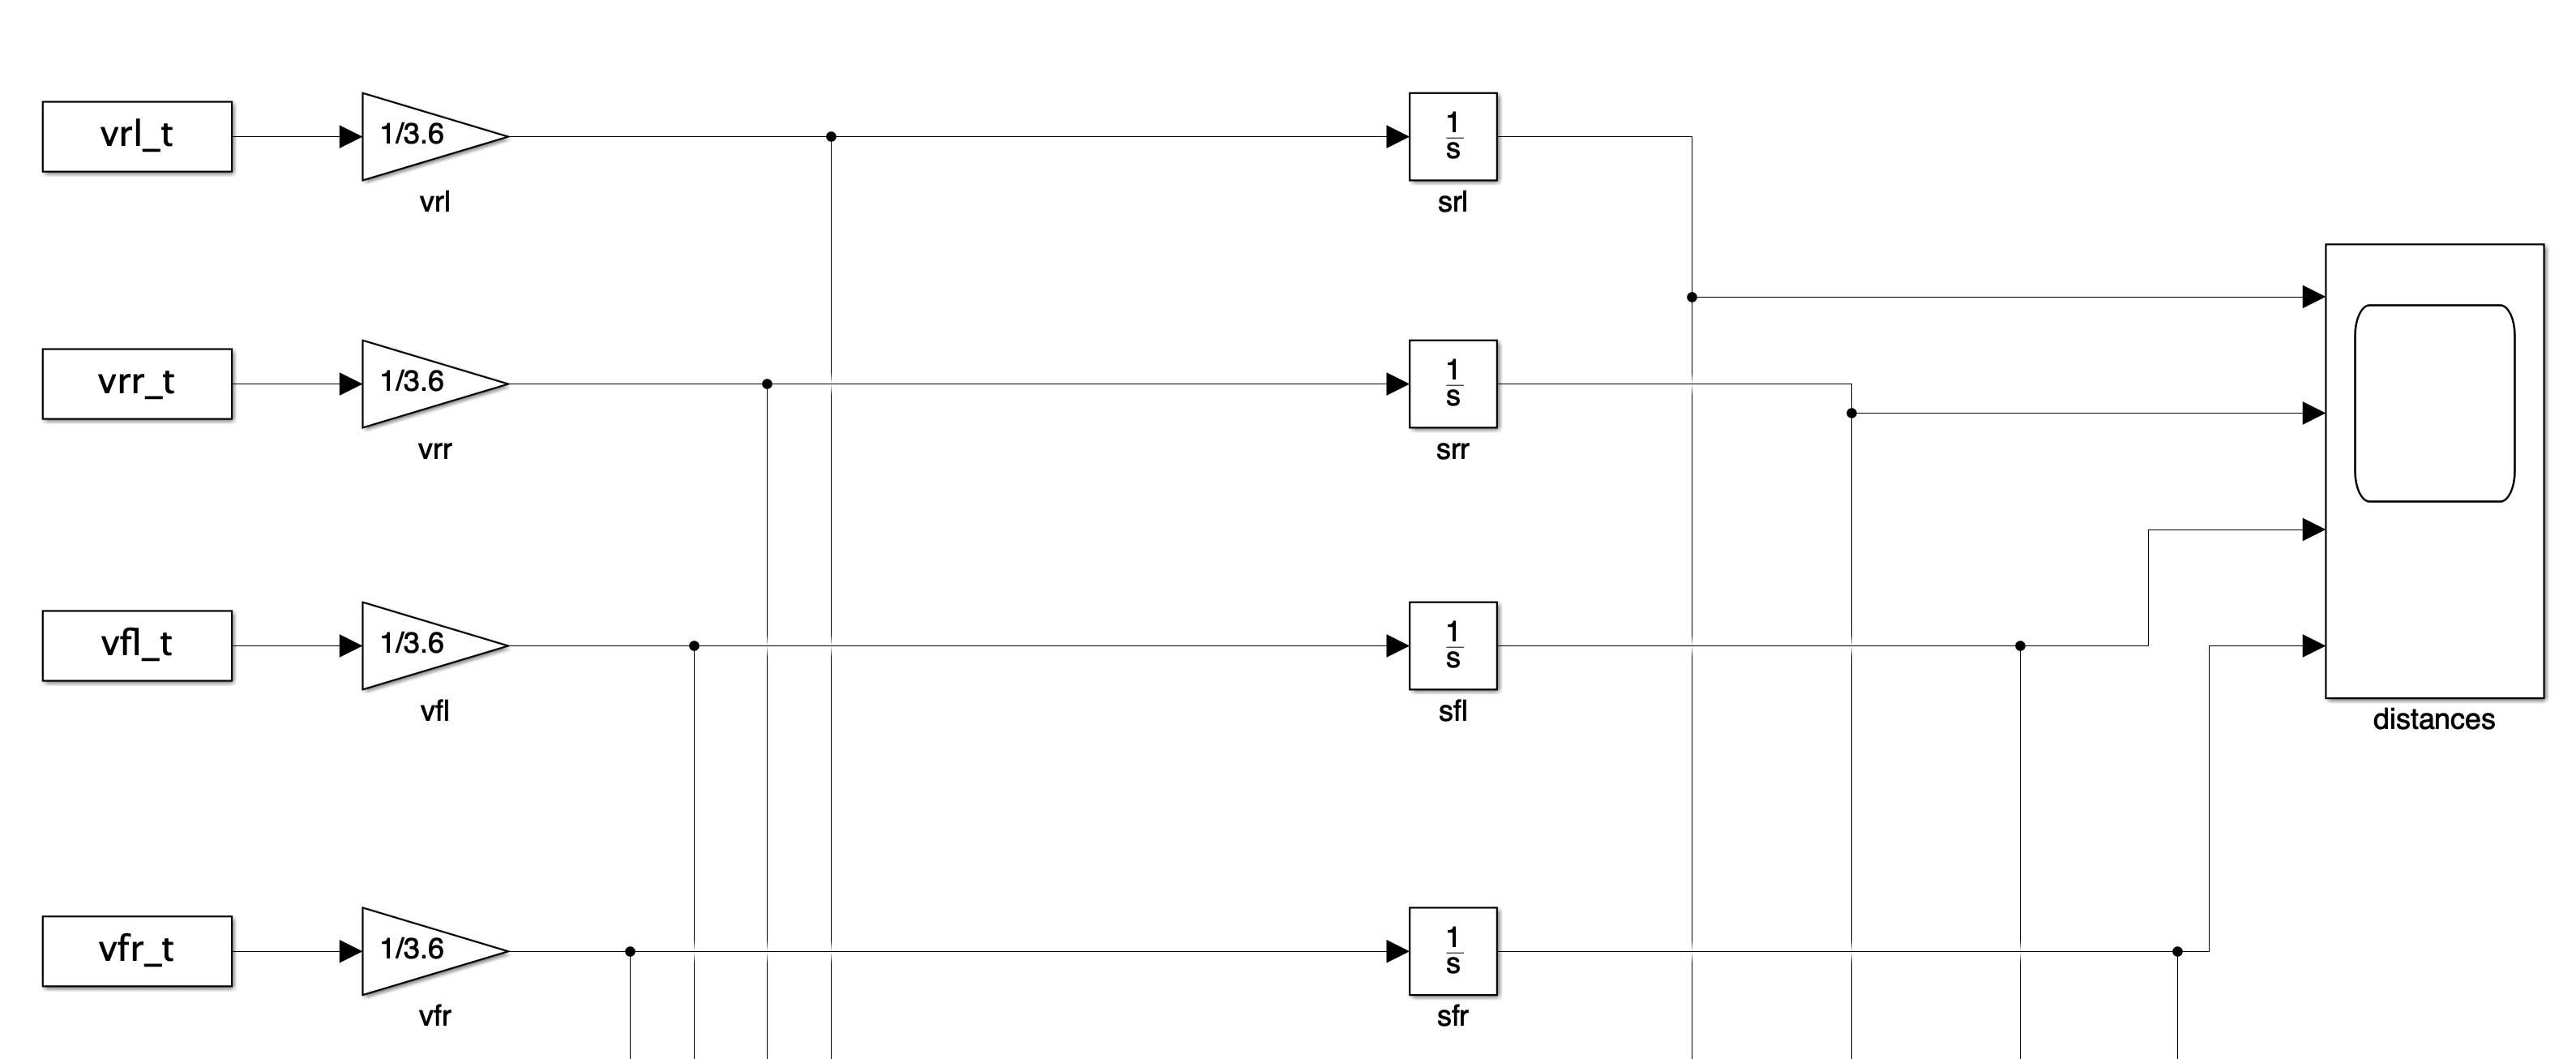
\includegraphics[width=1\linewidth]{../Graphiken/DrivingDistances1}
	\caption{Tire Driving distances}
	\label{fig:drivingdistances1}
\end{figure}
Das Ergebnis der Integration sind die Distanzen der einzelnen Reifen, die gegenüber der Zeit aufgetragen sind.\newpage
\begin{figure}[h!]
	\centering
	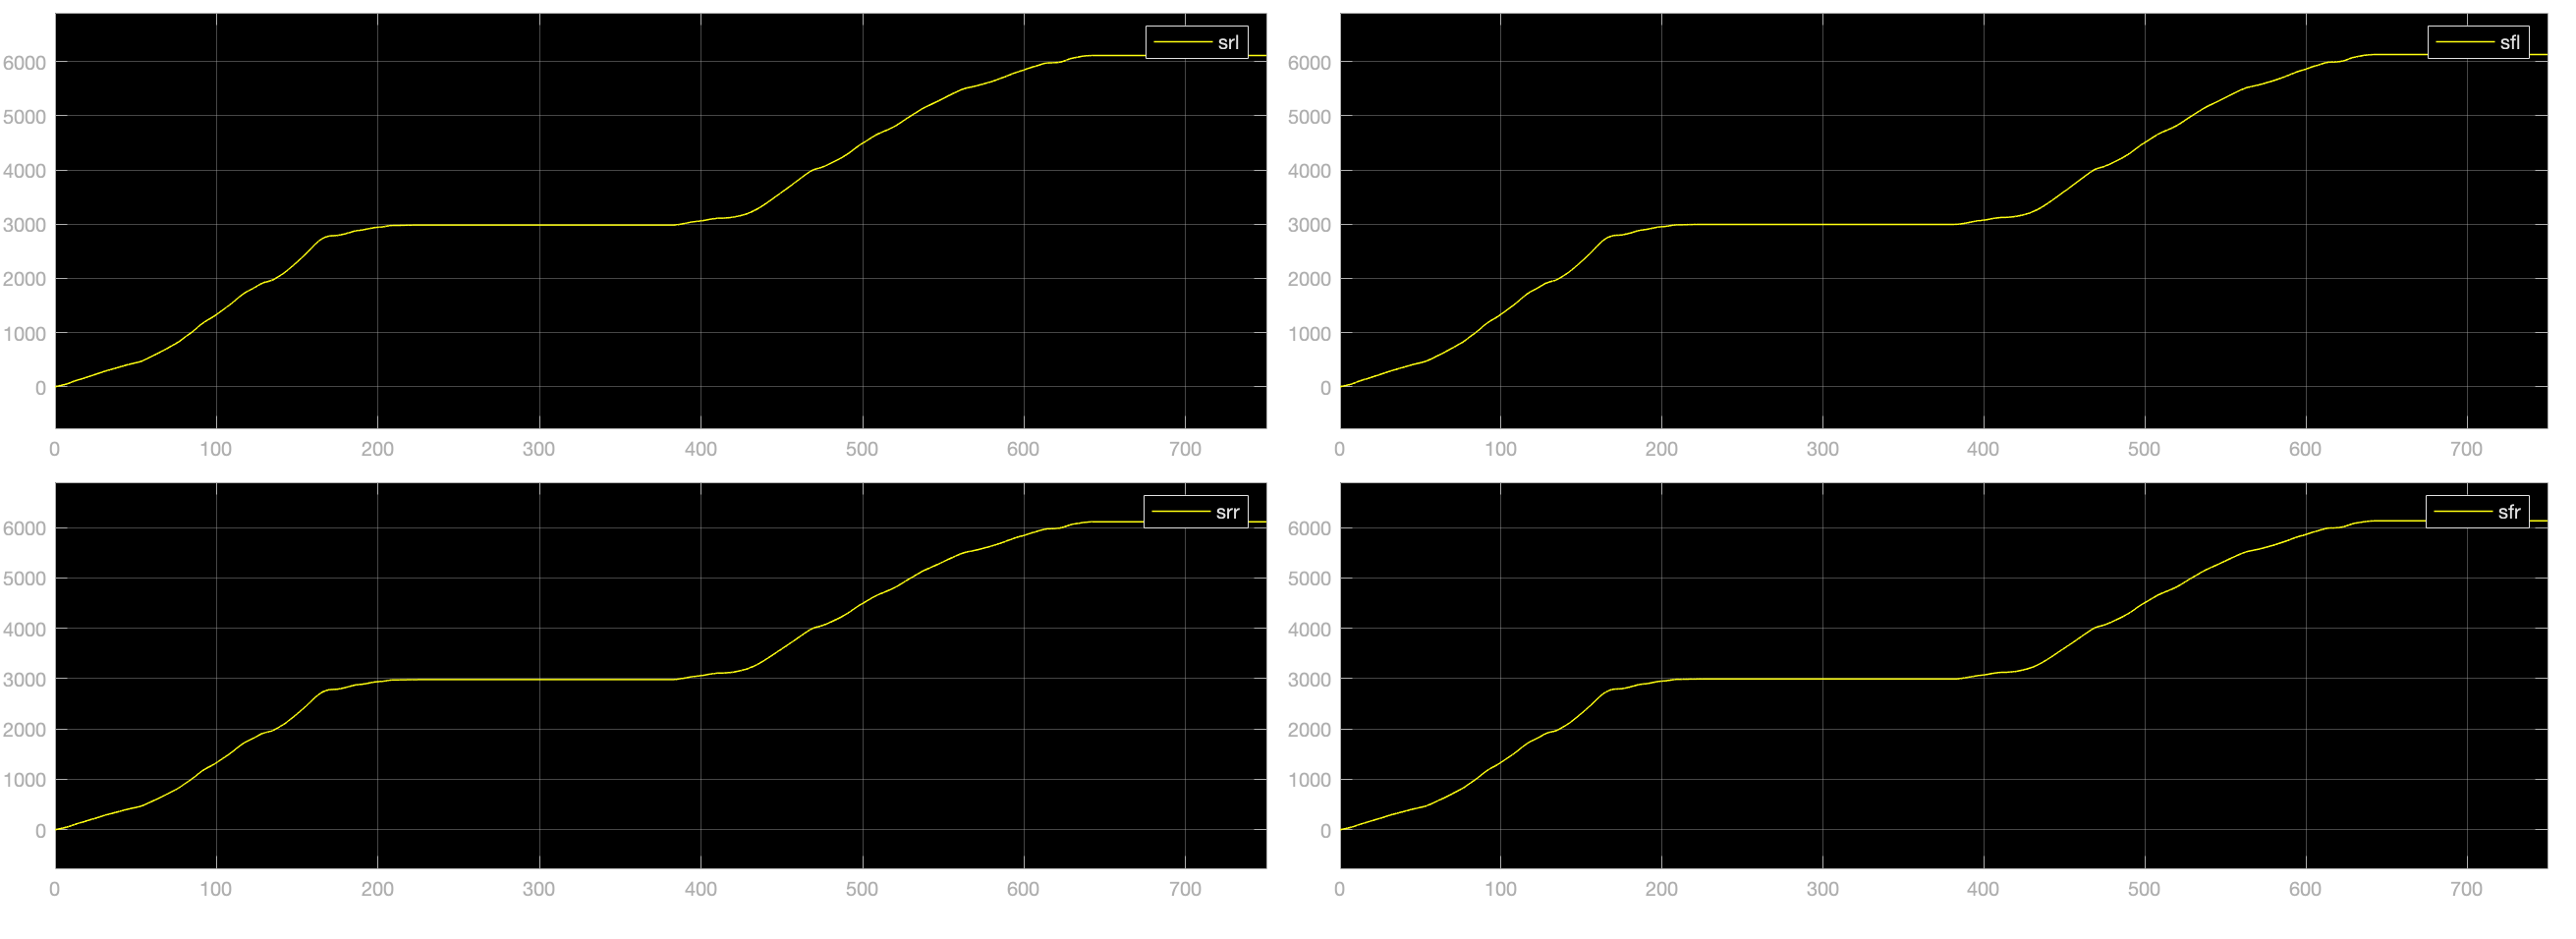
\includegraphics[width=1\linewidth]{../Graphiken/DrivingDistances}
	\caption{Tire Driving distances plot}
	\label{fig:drivingdistances}
\end{figure}



Für die Kurvenfahrt entsteht die folgende Datenaufzeichnung über die Reifendruckabweichungen.
\begin{figure}[H]
	\centering
	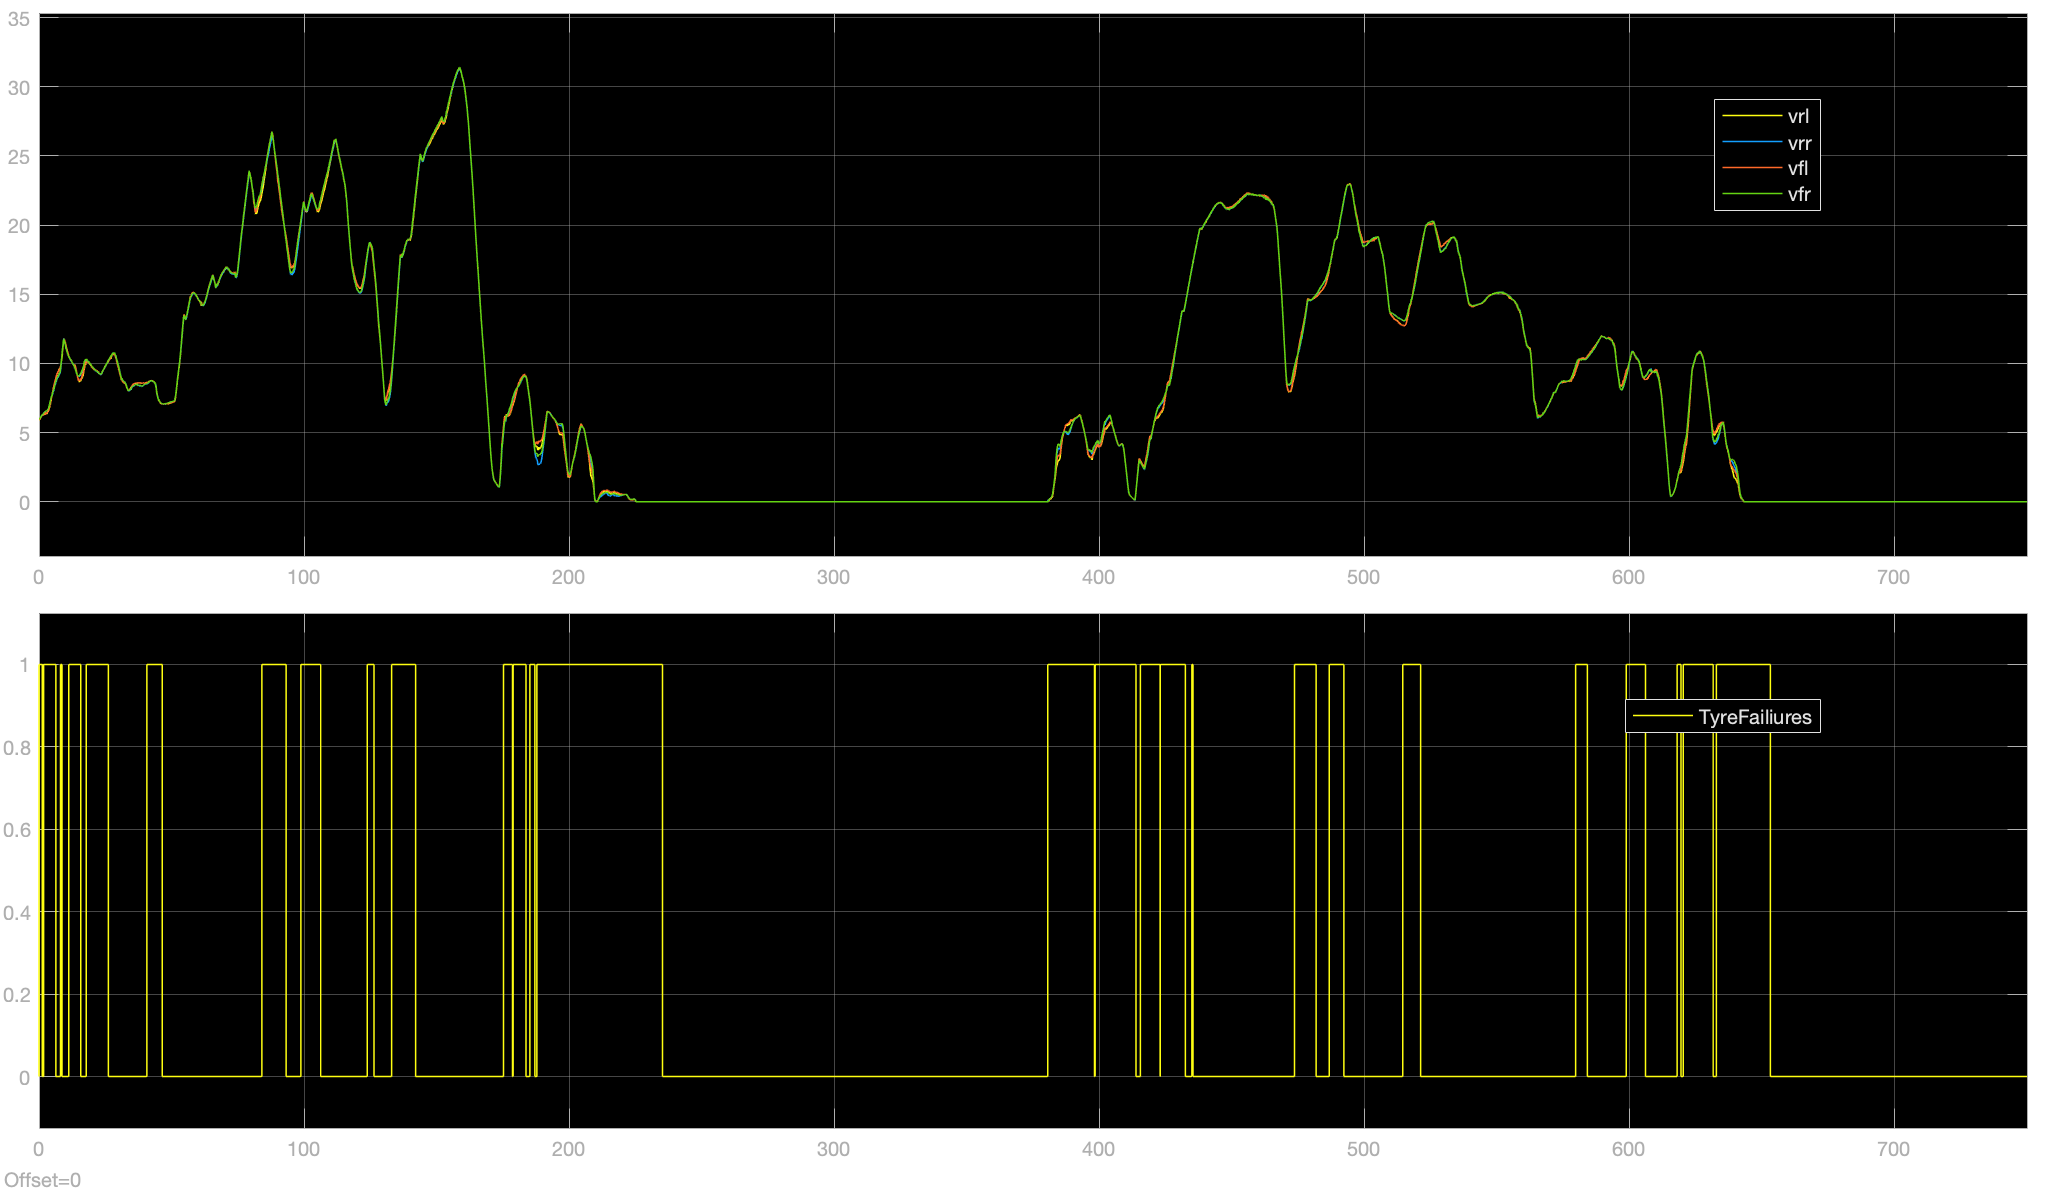
\includegraphics[width=0.95\linewidth]{../Graphiken/CurvesTireMonitor.png}
	\caption{Tire Monitor für Kurvenfahrt}
\end{figure}
Ein Wert von 1  entspricht der Beobachtung einer Imbalance und ein Wert von 0 entspricht keiner Anomalie.
\\
Wie berechnet wird, ob Imbalancen vorliegen wird in D4 thematisiert. Es werden viele Imbalancen gemessen, aber diese Implementation ist auch nicht für Kurvenfahrten geeignet. Weitere Ausführungen dazu finden bezüglich D13 statt.










	
	

	
	
	
	